
\documentclass[xcolor=pdftex,dvipsnames,table,mathserif,aspectratio=169]{beamer}
\usetheme{default}
\usetheme{metropolis}
\usepackage{minted}
\usepackage{mathtools}
\setbeamersize{text margin left=.3in,text margin right=.3in} 

\DeclarePairedDelimiter\abs{\lvert}{\rvert}%
\DeclarePairedDelimiter\norm{\lVert}{\rVert}%


%\usetheme{Darmstadt}
%\usepackage{times}
%\usefonttheme{structurebold}

\usepackage[english]{babel}
%\usepackage[table]{xcolor}
\usepackage{pgf,pgfarrows,pgfnodes,pgfautomata,pgfheaps}
\usepackage{amsmath,amssymb,setspace,centernot}
\usepackage[latin1]{inputenc}
\usepackage[T1]{fontenc}
\usepackage{relsize}
\usepackage{pdfpages}
\usepackage[absolute,overlay]{textpos} 


\newenvironment{reference}[2]{% 
  \begin{textblock*}{\textwidth}(#1,#2) 
      \footnotesize\it\bgroup\color{red!50!black}}{\egroup\end{textblock*}} 

\DeclareMathSizes{10}{10}{6}{6} 

\begin{document}
\title{Part 8: Program Evaluation (f):\\
Synthetic Control Methods}
\author{Chris Conlon}
\institute{Applied Econometrics}
\date{\today}

\frame{\titlepage}
\begin{frame}{Motivation: Recap}
Difference in Difference approaches have some drawbacks:
\begin{itemize}
\item We need to really believe \alert{parallel trends}
\begin{itemize}
\item Is $\Delta PA$ really a good counterfactual for  $\Delta NJ$?
\item Obvious question: why not pick $\Delta DE$ or $\Delta NY$?
\item Measured effect shouldn't change if our assumption is valid (but it probably will!)
\end{itemize}
\item With multiple treated individuals we can use 2WFE estimator
\begin{align*}
y_{it} = \beta X_{it} + \delta_i \cdot T_{it} +  \gamma_i + \gamma_t + u_{it}
\end{align*}
\vspace{-0.8cm}
\begin{itemize}
\item It assumes \alert{additivity} of FE $\gamma_i + \gamma_t$ are independent!
\item States have different baseline levels $\gamma_i$ but evolution over time is common $\gamma_t$.
\item Turns out it doesn't really generalize the diff-in-diff with $I > 2$ (Imai and Kim 2020).
\end{itemize}            
\end{itemize}              
\end{frame}


\begin{frame}{Motivation: Recap}
Matching Estimators had drawbacks too:
\begin{itemize}
\item We need to believe in as if random-assignment conditional on $X$
\item CIA: $\{Y_i(1), Y_i(0)\} \perp T_i | X_i$.
\end{itemize}
But we could use pretty flexible methods in constructing our matched controls:           
\begin{itemize}
\item We could try to match on multiple dimensions of $X$.
\item $k\text{\textendash}NN$, kernels, etc.
\end{itemize}
What if we could use ideas from \alert{matching} to better satisfy something like our \alert{parallel trends} assumptions?
\end{frame}

\section{Example: Abadie, Diamond, Hainmueller (2010)}

\begin{frame}{The Question}
In 1988 California passes anti-smoking Prop 99
\begin{itemize}
\item increased excise tax by 25 cents per pack, 
\item earmarked the tax revenues to health and anti-smoking education budgets and funded anti-smoking ads
\item led to indoor smoking bans in restaurants and bars city by city
\end{itemize}
 What was the effect on per capita cigarette sales?
 \begin{itemize}
 \item Already a bunch of pre-existing trends.
 \item What is a good control for California?
 \end{itemize}
 Use state-level data from 1970-2000.
\end{frame}

\begin{frame}{The Idea}
Use a convex combination of other states to construct a \alert{synethetic counterfactual California}.\\
\begin{itemize}
\item We observe $Y_{it}, X_{it},T_{it}$.
\item Assume only $i=1$ and $t > T_0$ are \alert{treated}.
\item Construct a \alert{donor pool} of potential controls subscripted by $j$.
\item Choose some \alert{weights} $w_j$ for each entity (state) in donor pool. How?
\begin{itemize}
\item Same $\mathbf{X_{1}} = \sum_j w_j \mathbf{X_{j}}$ as treated observations (like matching).
\item Same $\left({Y_{1,1},\ldots, Y_{1,T_0}} \right)= \sum_j w_j \cdot \left({Y_{j,1},\ldots, Y_{j,T_0}} \right)$ (like parallel trends).
\item Weights sum to one $\sum_j w_j = 1$ and maybe are non-negative (or not!)
\end{itemize}
\item Idea is to match all of the $X$'s and all of the $Y_{it}$'s in the \alert{pre-period}
\end{itemize}
\end{frame}

\begin{frame}{Covariate Balance}
\begin{center}
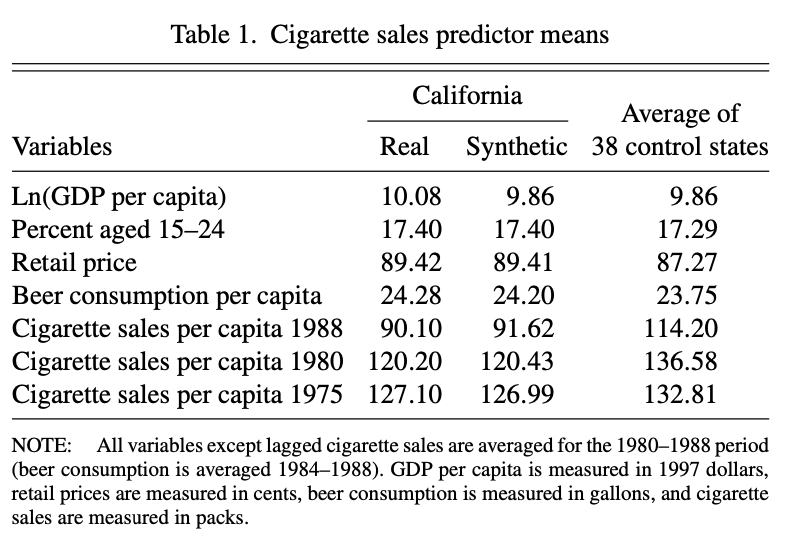
\includegraphics[width=4.5in]{./resources/abadie_1.png}
\end{center}
\end{frame}

\begin{frame}{Donor Weights}
\begin{center}
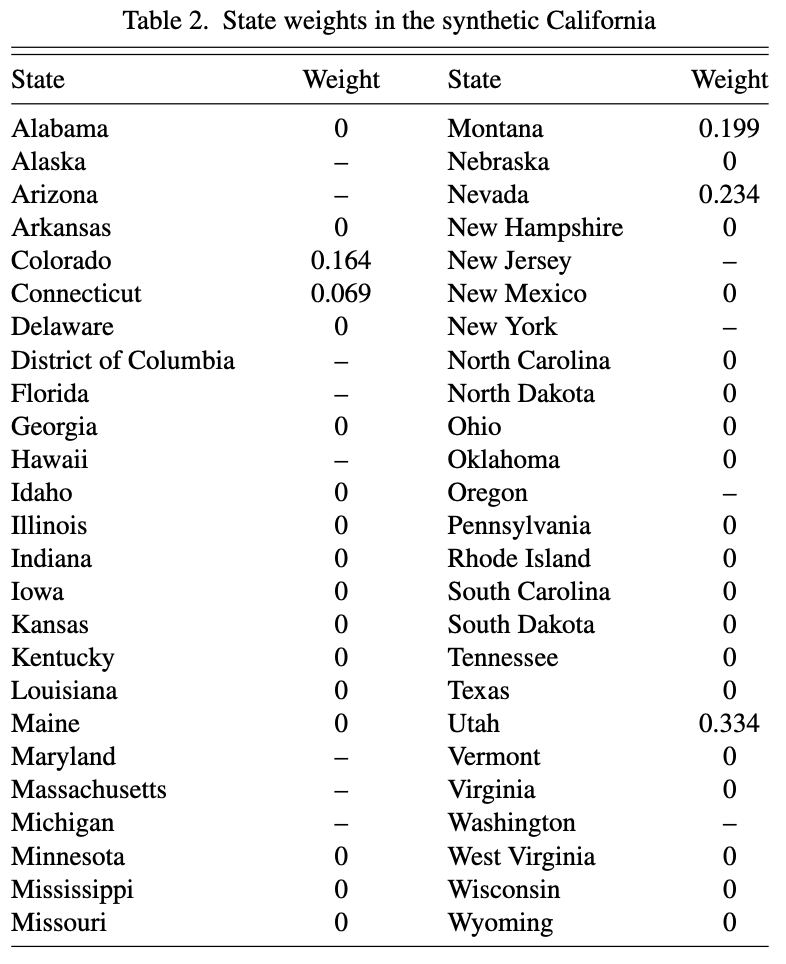
\includegraphics[width=2.5in]{./resources/abadie_2.png}
\end{center}
\end{frame}

\begin{frame}{Trend Check and Treatment Effects}
\begin{center}
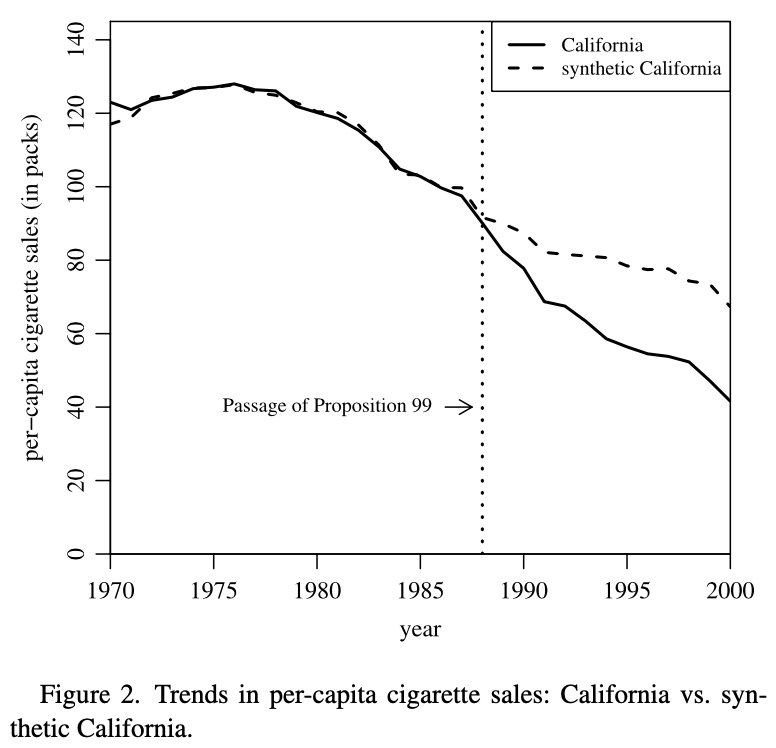
\includegraphics[width=2.75in]{./resources/abadie_3.png}
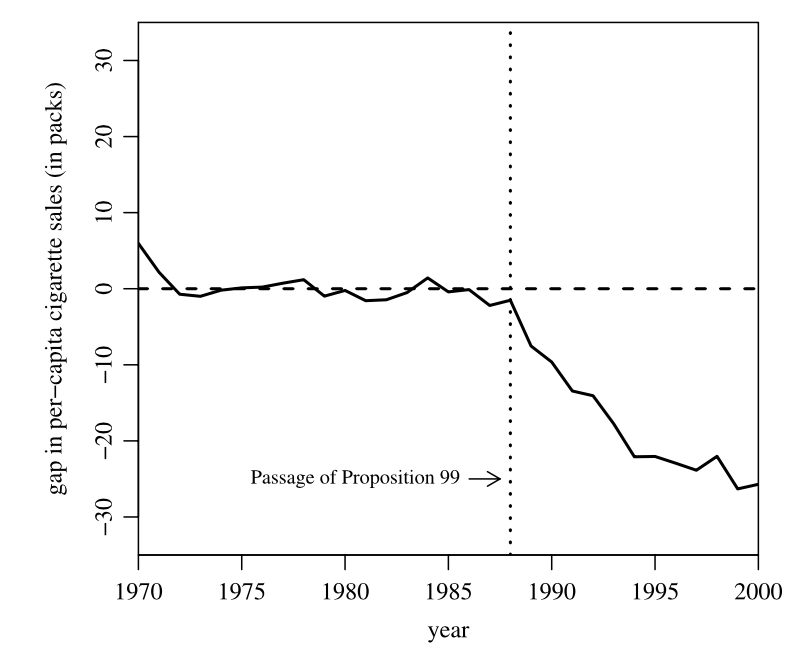
\includegraphics[width=2.75in]{./resources/abadie_4.png}
\end{center}
\end{frame}

\begin{frame}{But still some issues}
\begin{itemize}
\item How sensitive are weights estimates to different covariates?
\begin{itemize}
\item ``state-level measures of unemployment, income inequality, poverty, welfare transfers, crime rates, drug related arrest rates, cigarette taxes, population density, and numerous variables to capture the demographic, racial, and social structure of states''.
\end{itemize}
\item Can we run a \alert{placebo check}? Do we detect effects where we know there is a null effect?
\begin{itemize}
\item Put California in the donor pool.
\item Pick a state from the donor pool at pretend that receives the treatment after $T_0$
\item Choose $w_j$ following the synthetic control procedure.
\item Compute the treatment effects in the same way.
\item Repeat for all states in donor pool.
\item Compare \alert{mean-square prediction error} (MSPE) for $(Y_{1,1},\ldots,Y_{1,T_0})$
\item This doubles as \alert{inference}.
\end{itemize}
\end{itemize}
\end{frame}



\begin{frame}{Placebo Test}
\begin{center}
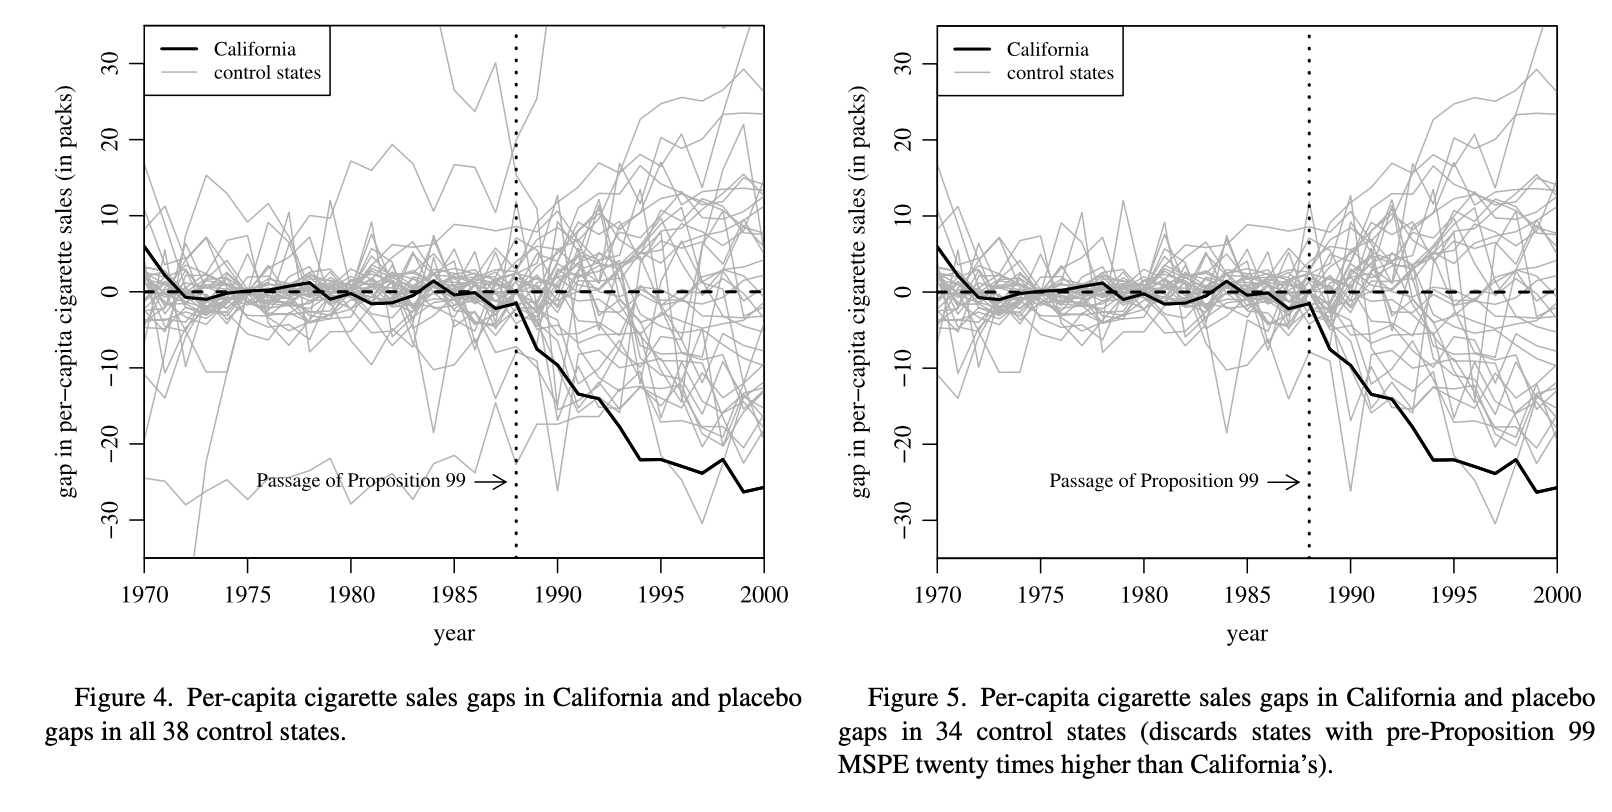
\includegraphics[width=5in]{./resources/abadie_5.png}
\end{center}
\end{frame}


\begin{frame}{More Placebo Tests: How unusual is the CA result?}
\begin{center}
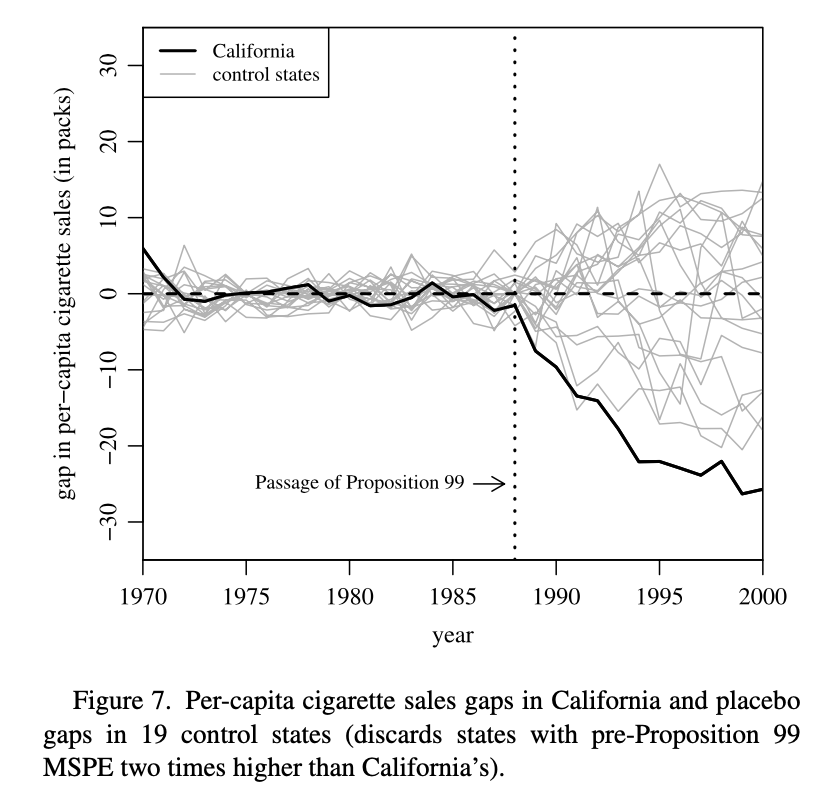
\includegraphics[width=2.75in]{./resources/abadie_6.png}
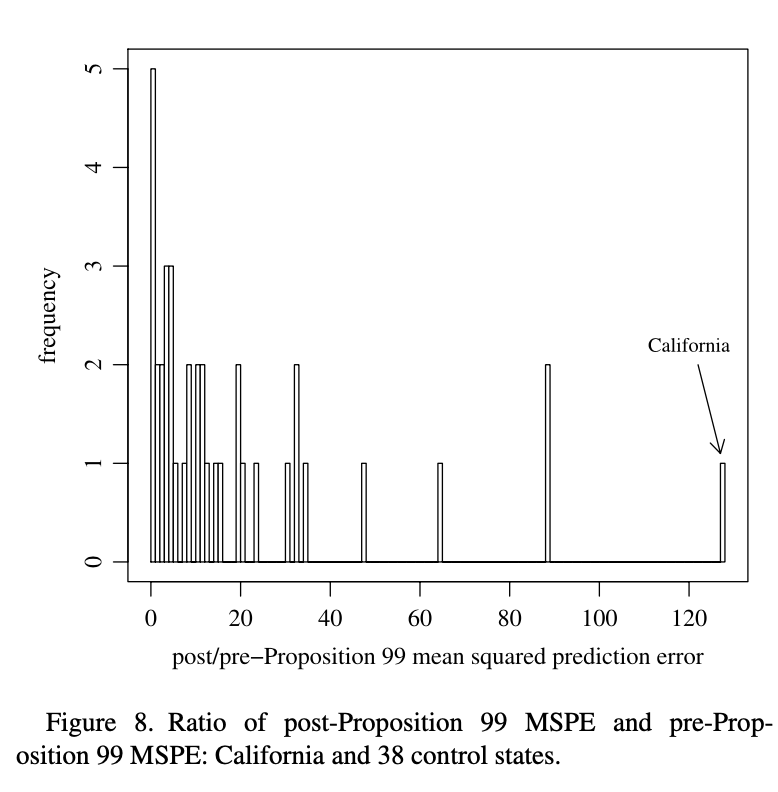
\includegraphics[width=2.75in]{./resources/abadie_7.png}
\end{center}
\end{frame}
\section{Thanks}






\end{document}
\item (for now) only first unit $i=1$ gets treated after $T_0$.
$T_{it}= \begin{cases}
1 & \text{ if } i=1, t \geq T_0 \\
0 & \text{ o.w.}
\end{cases}
$

